\chapter{Evaluation}
\label{cha:evaluation}

% TODO	DTLS

To support the development process and to measure code quality and
sustainability, unit tests were written. The test code coverage and the code
climate are also recorded. Our considerations of the research question
\enquote{How to handle a huge amount of \ac{IoT} devices?} are evaluated with
performance benchmarks. The interoperability of the different interfaces of the
server were benchmarked to analyze our considerations regarding to the research
questions covering the \ac{CoAP} implementation, the Rack interface, and
translations of headers and payloads between \ac{HTTP} and \ac{CoAP}.

\section{Unit Tests, Code Coverage, and Code Climate}
	
	The \ac{CoAP} library and client, the server (David), and the \ac{RD}
	implementation (core-rd) were developed mostly test-driven with RSpec
	\cite{rspec}. For the former some essential tests were ported to and new
	ones were written with RSpec. For the other two components RSpec was used
	exclusively. Although it offers some features supporting \ac{BDD}, we used
	RSpec only to write \ac{DRY} specifications of the codes functionality. The
	\acl{TDD} of the \ac{RD} showed that RSpec can seamlessly be used for the
	development of \ac{CoAP} applications with \ac{Rails}.

	The test coverage is determined by Coveralls, a web service that gets
	coverage measurement values from test runs in the \ac{CI} system using the
	simplecov gem\footnote{\url{https://rubygems.org/gems/simplecov}}. The
	results are prepared for easy analyzing by developers and displayed
	publicly. We used CodeClimate -- another similar service -- for measuring
	for example the complexity of methods by counting conditional branches and
	method calls. Classes and modules are classified by their complexity into
	categories from A (best) until F (worst). A code climate score (between 0.0
	and 4.0) is computed from that information that indicates code quality.

	% TODO	Update numbers!
	% TODO	Graphs or screenshots!

	For the fork of the coap library gem, the code climate score was raised
	from 0.74 to 2.66\footnote{\urlClimateCoap} and the test coverage from
	88.19\% to 93.06\%\footnote{\urlCoverageCoap} (although the total count of
	code lines increased from about 1270 to 1900). The test coverage for
	core-rd -- the \ac{RD} draft \cite{rd} implemented in Rails -- is about
	90.01\%\footnote{\urlCoverageCoreRd}, the CodeClimate score is
	3.37\footnote{\urlClimateCoreRd}. The source code of David scores
	3.57\footnote{\urlClimateDavid} on CodeClimate and has a test coverage of
	92.94\%\footnote{\urlCoverageDavid}.

\section{Benchmarking}

	We benchmarked the performance and interoperability of the developed server
	software. The performance was tested by measuring the handled \acl{RPS} in
	different Ruby \acp{VM} and with Rack and \ac{Rails}. For the
	interoperability, several tests were conducted per interface.

	\subsection{Performance}
	\label{cha:evaluation:performance}

		We tested the requests David handles (receives, parses, processes, and
		answers) per second with Rack and \ac{Rails} applications simply
		returning a plain \enquote{Hello World!} string. This \emph{\acl{RPS}}
		value is measured with a number of concurrent clients that increases
		from 10 to 10,000 (by 10 below 100, 100 below 1,000 and 1,000 below
		10,000) simulated with \emph{Cf-CoAPBench}
		1.0.0-M3\footnote{\url{https://github.com/eclipse/californium.tools/tree/1.0.0-M3/cf-coapbench}}.
		We use a server running on loopback instead of a physical network and
		the different Ruby \acp{VM} mentioned below. The exact versions are
		noted as output from the \texttt{ruby -v} command. Benchmarking for
		each concurrency value is performed for 30 seconds. The average value
		of three subsequent runs is recorded. After each benchmark, we wait 15
		seconds. At the beginning of the testing of each \ac{VM} or framework,
		a 60 seconds warmup is done. The benchmark system is a notebook with a
		Core i7-3520M \ac{CPU} and 16 GiB of \ac{RAM} running Arch Linux.
		Benchmarks were conducted on the core repository linux kernel version
		3.18.6-1 without further tuning. We only increased the maximum number
		of open file descriptors to enable 100,000 open \acs{UDP} sockets. The
		\ac{CPU} supports Hyper-Threading and regularly runs at 2.9 GHz and 3.9
		GHz with only one active core. Server processes are started with
		\texttt{rackup} and a framework specific rackup configuration file
		(\href{https://github.com/nning/david/blob/0.4.1/benchmarks/rackup/rack.ru}{\texttt{benchmarks/rackup/rack.ru}}
		and
		\href{https://github.com/nning/david/blob/0.4.1/benchmarks/rackup/rails.ru}{\texttt{benchmarks/rackup/rails.ru}})
		and the benchmarking uses the script at
		\href{https://github.com/nning/david/blob/0.4.1/benchmarks/stress.sh}{\texttt{benchmarks/stress.sh}}.
		The server release
		\href{https://github.com/nning/david/tree/0.4.1}{\texttt{0.4.1}} is
		used. It was planned to also test Rubinius 2.5.2 as a Ruby \ac{VM} but
		because of a deadlock issue that could not be fixed yet, this benchmark
		is postponed for now.

		\begin{enumerate}
			\item \ac{MRI} 2.2.0p0\\
				(2014-12-25 revision 49005)
			\item \ac{MRI} 2.3.0dev\\
				(2015-02-12 trunk 49574)
			\item JRuby 1.7.19\\
				(1.9.3p551) 2015-01-29 20786bd on OpenJDK 64-Bit Server VM
				1.7.0\_75-b13 +jit
			\item JRuby 9.0.0.0-pre1\\
				(2.2.0p0) 2015-01-20 d537cab OpenJDK 64-Bit Server VM
				24.75-b04 on 1.7.0\_75-b13 +jit
			% \item Rubinius 2.5.2\\
			% 	(2.1.0 8fd046f3 2015-01-26 3.5.1 JI)
		\end{enumerate}

		The garbage collection of both \ac{MRI} versions was tuned by setting
		environment variables to increase the memory allocation maximum (128M)
		and to prepare a certain amount of free slots after starting the
		\ac{VM} (200000). JRuby has been configured to use the Server \ac{JVM}.
		\autoref{lst:evaluation:env} shows the environment variables and their
		values.

		\begin{figure}
			\begin{lstlisting}[gobble=8,caption={Performance benchmark environment variables},label=lst:evaluation:env]
				export RUBY_GC_MALLOC_LIMIT=134217728
				export RUBY_GC_HEAP_FREE_SLOTS=200000
				export JRUBY_OPTS="--server"
			\end{lstlisting}
		\end{figure}

		We benchmarked Reel \cite{reel} on the same hardware with 1,000 and
		10,000 concurrent clients to get a reference value to a \ac{HTTP}
		server based on a very similar concurrency model and also on
		\emph{Celluloid} and \emph{Celluloid::IO}. It achieved 3,391.6 \ac{RPS}
		at 1,000 and 3,414.4 \ac{RPS} at 10,000 concurrent connections running
		in \ac{MRI} 2.2.0p0.

		We also tried to perform a performance benchmark with David running on
		an \emph{Ubiquiti EdgeMAX Lite} router, as it is quite customizable and
		comparable to common customer router hardware. However, we could not
		get the performance benchmark running even after extensive experiments.
		See \autoref{cha:rawdata:ubiquiti} for installation instructions on
		that hardware and a documentation of the steps taken by us.

		\begin{figure}
			\begin{center}
				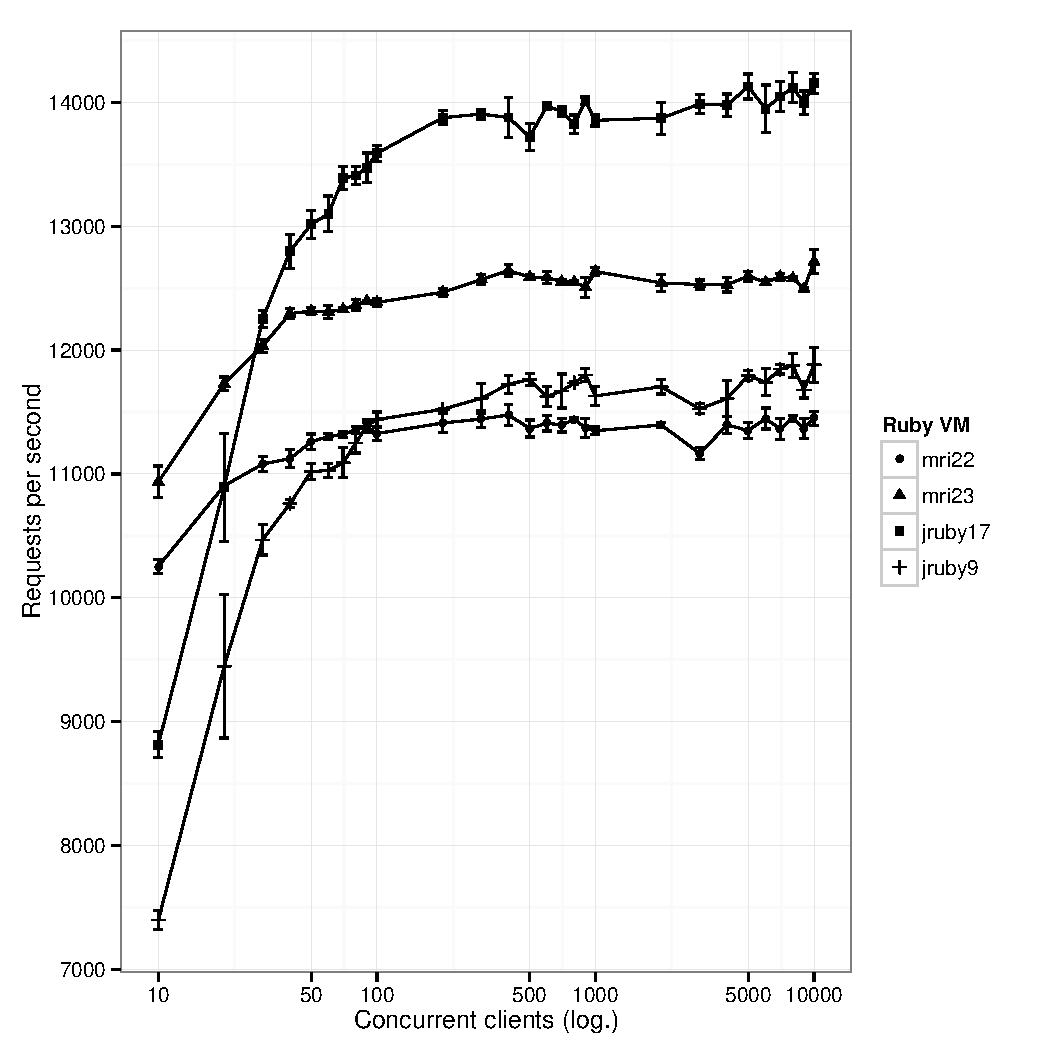
\includegraphics[width=\textwidth]{images/throughput-vms-rack.pdf}
			\end{center}
			\caption{Throughput by Ruby \ac{VM} with Rack}
			\label{img:evaluation:throughput-vms-rack}
		\end{figure}

		\begin{figure}
			\begin{center}
				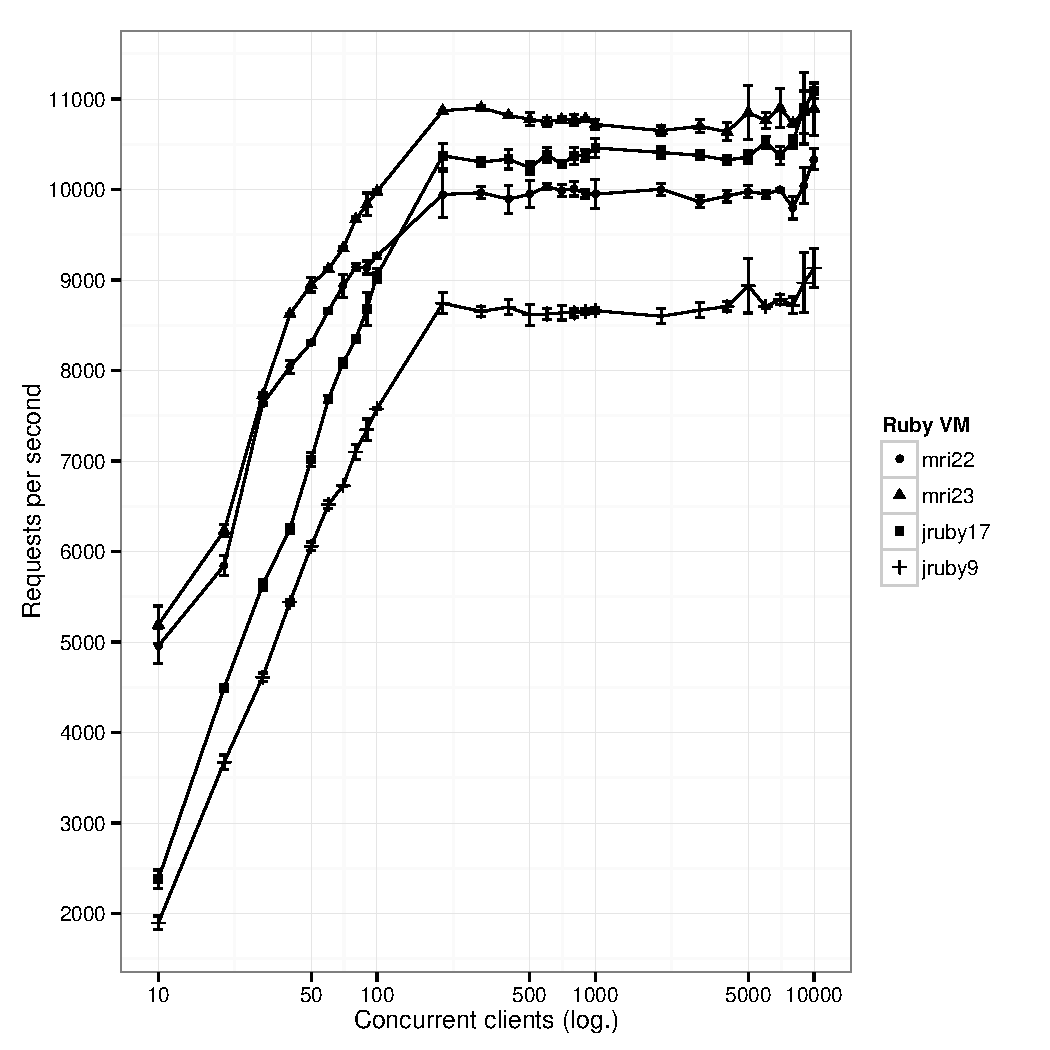
\includegraphics[width=\textwidth]{images/throughput-vms-rails.pdf}
			\end{center}
			\caption{Throughput by Ruby \ac{VM} with \ac{Rails}}
			\label{img:evaluation:throughput-vms-rails}
		\end{figure}

		% TODO	Error bars.
		\begin{figure}
			\begin{center}
				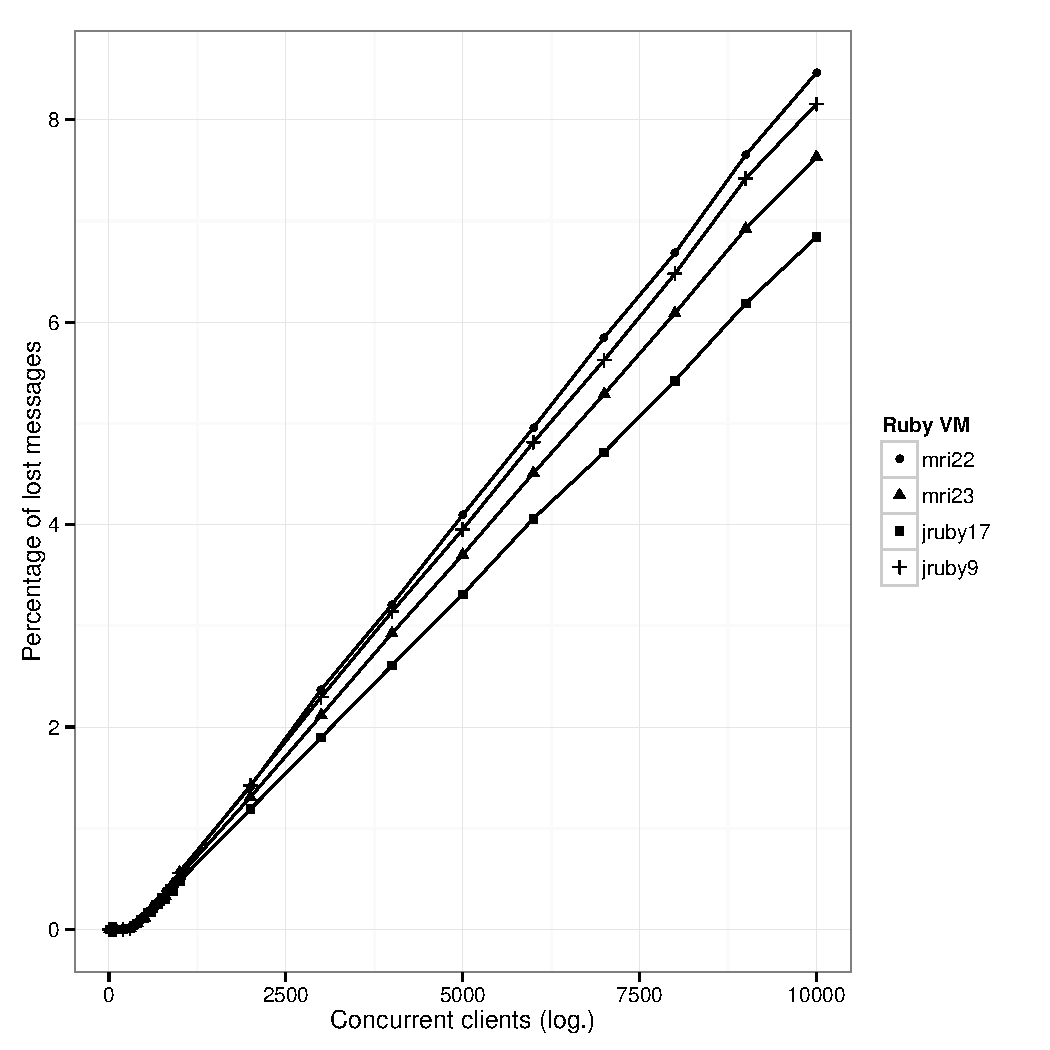
\includegraphics[width=\textwidth]{images/loss-vms-rack.pdf}
			\end{center}
			\caption{Message timeouts by Ruby \ac{VM} with Rack}
			\label{img:evaluation:loss-vms-rack}
		\end{figure}

		\begin{figure}
			\begin{center}
				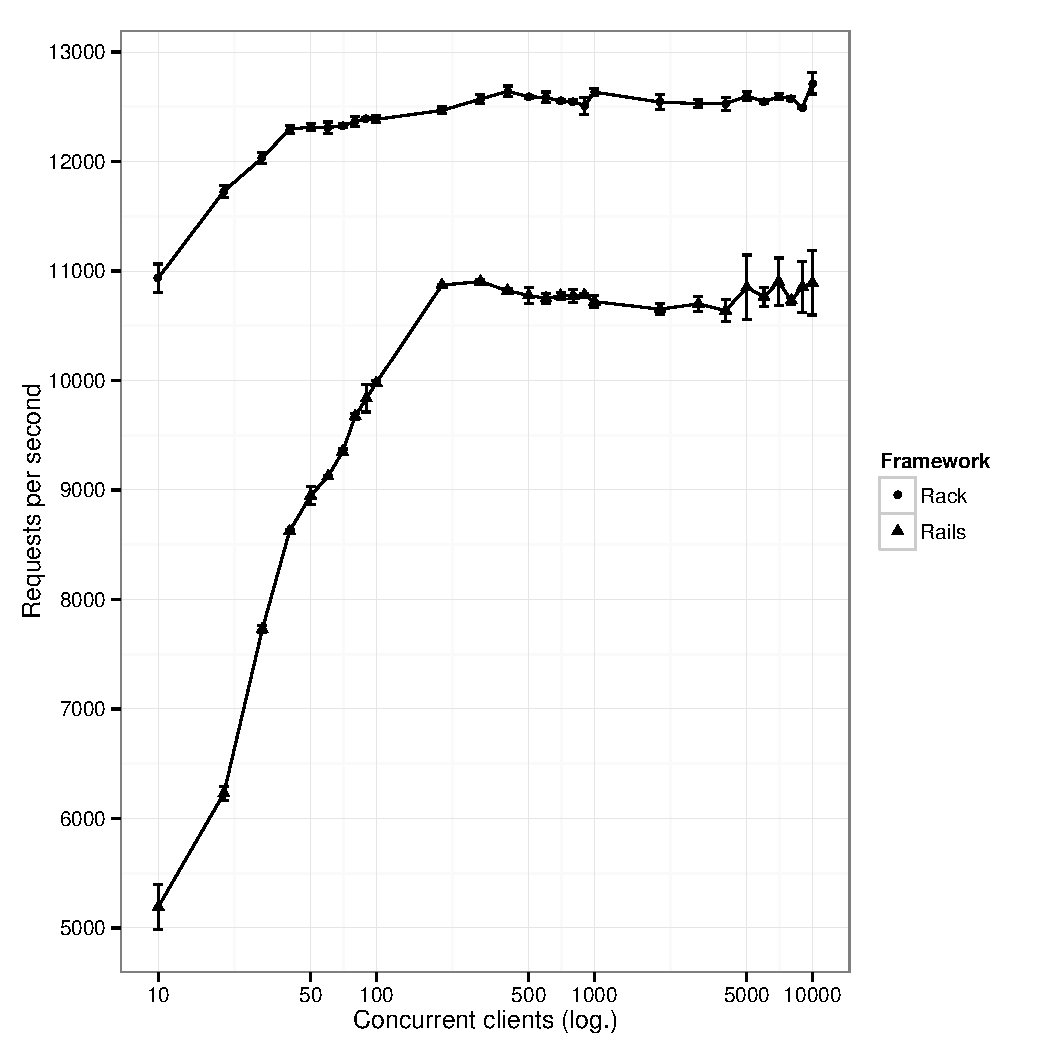
\includegraphics[width=\textwidth]{images/throughput-frameworks-mri23.pdf}
			\end{center}
			\caption{Throughput by Framework in \ac{MRI} 2.3.0dev}
			\label{img:evaluation:throughput-frameworks-mri23}
		\end{figure}

		\begin{figure}
			\begin{center}
				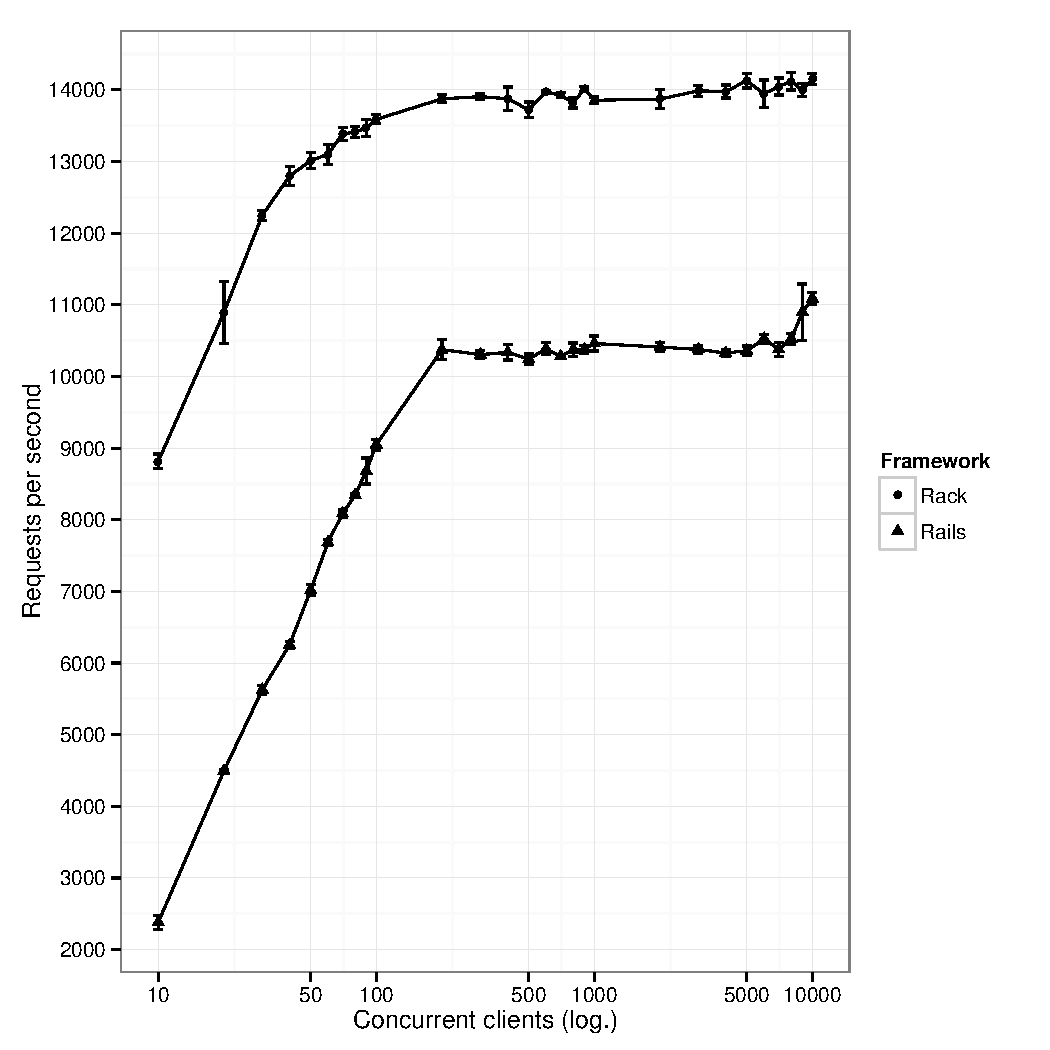
\includegraphics[width=\textwidth]{images/throughput-frameworks-jruby17.pdf}
			\end{center}
			\caption{Throughput by Framework in JRuby 1.7.19}
			\label{img:evaluation:throughput-frameworks-jruby17}
		\end{figure}

		The rate of \acl{RPS} stays quite stable with rising numbers of
		concurrent clients in any Ruby \ac{VM} (see
		\autoref{img:evaluation:throughput-vms-rack} and
		\ref{img:evaluation:throughput-vms-rails}). In JRuby 1.7.19 throughput
		rates of about 14,000 \acl{RPS} are possible. \ac{MRI} 2.3.0dev handles
		about 12,500 \acl{RPS}. In \ac{MRI} with Rack, the peak throughput is
		reached with quite a low number of concurrent clients compared to
		\ac{Rails}. Until 200 concurrent clients, the \ac{Rails} framework
		overhead in the event loop seems to be the bottleneck. A decrease in
		throughput with high numbers of concurrent clients does not occur. In
		JRuby the throughput with Rack and \ac{Rails} in relation to concurrent
		clients runs quite comparable with between 6,500 and 3,500 \acl{RPS}
		deviation. With Rails JRuby 1.7.19 does not perform as good as \ac{MRI}
		2.3.0dev especially with lower numbers of concurrent clients (see
		\autoref{img:evaluation:throughput-frameworks-mri23} and
		\ref{img:evaluation:throughput-frameworks-jruby17}). In JRuby
		9.0.0.0-pre1 the server has a surprisingly low throughput especially
		with \ac{Rails} and mainly with low numbers of concurrent clients.

		\autoref{img:evaluation:loss-vms-rack} shows the message loss through
		timeouts waiting for responses by Ruby \ac{VM} with Rack. With 300
		concurrent clients stressing the server, timeouts when waiting
		for responses start to occur. This happens throughout different
		\acp{VM} and with different numbers of total messages received during a
		30 seconds stressing period. The timeout rates rise with the number of
		concurrent clients to a maximum of about 9\% at 100,000 concurrent
		clients (\ac{MRI} 2.2.0p0 serving a \ac{Rails} application). We tried
		increasing the \ac{UDP} receive buffer up to 1 MiB (default was 208
		KiB) via the sysctl flag \texttt{net.core.rmem\_max} but could not
		observe a descrease in message loss. It raises the question if
		\emph{Cf-CoAPBench} includes the exponential back-off mechanism for
		retransmissions of confirmable messages to achieve congestion control
		(see section 4.2 of \cite{coap}). We could not find any indication for
		this (see
		\href{https://github.com/eclipse/californium.tools/blob/1.0.0-M3/cf-coapbench/src/main/java/org/eclipse/californium/tools/coapbench/VirtualClient.java#L113}{line
		113 of VirtualClient}).

		Plots showing the message timeouts by Ruby \ac{VM} with \ac{Rails} and
		the throughput by framework in \ac{MRI} 2.2.0p0 and JRuby 9.0.0.0-pre1
		are included in the appendix (see \autoref{cha:rawdata:performance}).

	\subsection{Interoperability}
	\label{cha:evaluation:interoperability}

		The interoperability of the server has to be evaluated especially
		regarding to the two interfaces with other software. It interfaces via
		\ac{CoAP} with other nodes and via Rack with web frameworks. So test
		cases are needed for both interfaces that let us specify the
		interoperability capabilities of the implemented software. The
		\ac{ETSI} \ac{CoAP} Plugtests \cite{etsi-plugtests} are specifications
		for interoperability tests previously conducted within the community of
		\ac{CoAP} developers. They are both valuable for testing the \ac{CoAP}
		and Rack interoperability. It is possible to analyze the following
		questions utilizing implementations of this test specifications.
		However, some of the test cases are not compatible to the
		specifications of the latest \ac{CoAP} version \cite{coap}.
		\texttt{TD\_COAP\_CORE\_11} for example demands a missing token option
		on a response. Others are not specified detailed enough.
		\texttt{TD\_COAP\_CORE\_13} for example does not require the server to
		actually handle the \ac{URI}-Query options.

		\begin{enumerate}
			\item Which \ac{CoAP} features are supported and possible to
				implement in an application hosted by the server?
			\item How compatible is the Rack interface implementation of
				the server to different web frameworks? 
			\item How compatible is the \ac{CoAP} implementation of the
				server to different \ac{CoAP} clients?
		\end{enumerate}

		Data for answering these questions is gained by means of
		implementing the Plugtests as RSpec tests. Most Plugtests have been
		implemented, but not all. We had to concentrate on the tests for the
		most important aspects regarding to the research questions. Currently,
		only the \ac{CoAP} protocol tests 1-13 (without 9) are implemented (see
		section 7.1 of \cite{etsi-plugtests}). \texttt{TD\_COAP\_CORE\_09} is
		not implemented, because the server does not support separate
		responses. From the optional test case set we implemented the
		block-wise transfers tests \texttt{TD\_COAP\_BLOCK\_01} and
		\texttt{TD\_COAP\_BLOCK\_02} as well as the first three observe tests.
		Block-wise transfers with \texttt{PUT} and \texttt{POST} are not
		supported by the server and therefore also not tested (\ac{ETSI}
		Plugtests \texttt{TD\_COAP\_BLOCK\_03} and
		\texttt{TD\_COAP\_BLOCK\_04}). The same applies to server observe
		deregistration detection (tests \texttt{TD\_COAP\_OBS\_04} and
		\texttt{TD\_COAP\_OBS\_05}).

		The automatic provisioning of the Resource Discovery only works with
		\ac{Rails}. Therefore the Plugtests regarding to the \ac{CoRE} Link
		Format were omited for this test series. Tests similar to the \ac{CoRE}
		Link Format test cases have been implemented before the evaluation
		phase as unit and integration tests (see for example
		\href{https://github.com/nning/david/blob/0.4.3/spec/resource\_discovery\_spec.rb}{\texttt{spec/resource\_discovery\_spec.rb}
		in the david repository}). We tested different \ac{Rails} applications
		enabling the automatic provisioning of Resource Discovery with the
		\emph{\ac{CoAP} crawler client} on \url{http://coap.me} and there was
		no indication of problems in the \ac{RD} middleware implementation.
		Tested applications were the dummy used for automatic testing of David
		(see
		\href{https://github.com/nning/david/tree/0.4.3/spec/dummy}{spec/dummy}),
		the core-rd application, and a prototype \ac{Rails} application used
		for the development of David. The interoperability of the \ac{RD}
		application is not tested as we could not find any \ac{RD} client
		implementation or test cases.
		
		\subsubsection{Features}

			% TODO	More How? More results?

			During the implementation of the Plugtests, test cases occured that
			are impossible to be realized because of lacking server support for
			certain features. All of those shortcomings were already known.
			Separate responses (see section 5.2.2 of \cite{coap} and test
			TD\_COAP\_CORE\_09 of \cite{etsi-plugtests}) are one example.
			Another one is the lack of support for block-wise transfers for
			incoming messages (see \ac{ETSI} Plugtests
			\texttt{TD\_COAP\_BLOCK\_03} and \texttt{TD\_COAP\_BLOCK\_04}).
			The token generation of the client library has been revised during
			the implementation of the test \texttt{TD\_COAP\_CORE\_11}. We also
			found regressions in the server implementation regarding to the
			support for block-wise transfers and observe. As the \ac{Rails}
			application is used solely as an \ac{API}, we removed all
			stylesheet or JavaScript asset related gems and paths from the
			source tree.

		\subsubsection{Rack}
		\label{cha:evaluation:interoperability:rack}

			% TODO	How? More results?

			We implemented the Client side of the Plugtests as RSpec tests and
			the server side with means of different Rack based web frameworks.
			A list of the tested frameworks and their versions is shown in
			\autoref{table:evaluation:interoperability:rack}.
			\autoref{table:background:rack} contains an exhaustive list of
			frameworks and their download locations. The framework specific
			applications are to be found in
			\href{https://github.com/nning/david/tree/0.4.3/lib/david/etsi}{the
			\texttt{lib/david/etsi} folder of the david repository}.

			\begin{table}[H]
				\begin{center}
					\begin{tabular}{l|l}
						Framework		& Version \\
						\hline
						Grape			& 0.10.1 \\
						Hobbit			& 0.6.0	 \\
						NYNY			& 2.2.1	\\
						Pure Rack		& \\	 
						Sinatra			& 1.4.5	\\
						\acl{Rails}		& 4.2.0	\\
					\end{tabular}
				\end{center}
				\caption{Rack based web frameworks tested on interoperability}
				\label{table:evaluation:interoperability:rack}
			\end{table}

			When designing the \ac{HTTP} status code mappings and explicitly
			returning a \ac{CoAP} response code by using a Float,
			\texttt{\#to\_i} was not called on the status. At the time of
			Rack interface interoperability testing, it became obvious
			that returning Float status codes does not work anymore from any
			framework. So two changes were made to the server code. First it is
			possible that \ac{CoAP} response codes are used in the style of
			\ac{HTTP} response codes (for example \emph{205} meaning
			\ac{CoAP} \emph{2.05}. However, with the designed mapping in place,
			\emph{204} for example would be interpreted as \ac{HTTP} \emph{204
			No Content} and mapped to \ac{CoAP} \emph{2.05 Content}. Therefore,
			a possibility to configure the status code mapping as minimal as
			possible was implemented. Currently only \ac{HTTP} \emph{200 OK}
			maps to \ac{CoAP} \emph{2.05 Content} in this mode. The Rack
			environment option \texttt{MinimalMapping} can be set to true to
			activate the minimal mapping. The second change affects the method
			in Rack code that calls \texttt{\#to\_i} on the status returned by
			the framework. This method was monkey-patched to omit calling
			\texttt{\#to\_i} on the status if it is an instance of the Float
			class. \emph{Grape} and \emph{Sinatra} call \texttt{\#to\_i} on the
			status by themselves. \emph{Grape} uses \texttt{Rack::Request},
			which calls \texttt{\#to\_i} on initialization and in the
			\emph{Sinatra} code it is called in different places. With these
			frameworks \ac{CoAP} response codes as Integers have to be used for
			now. Wrapping the status in a \ac{CoAP} status object instance is
			not a trivial solution. The response code \emph{205} for example in
			\ac{HTTP} means \emph{Reset Content} and results in clearing the
			body and headers in \emph{Grape}. The wrapper object would have to
			actually return an Integer on call of \texttt{\#to\_i}. Code like
			\texttt{status = status.to\_i} (like in \texttt{Rack::Response})
			would erase the \ac{CoAP} response code information. Out of the
			tested frameworks, only \emph{Hobbit}, Pure Rack and Rails support
			the \ac{CoAP} response codes as Floats.

		\subsubsection{\ac{CoAP}}

			We conduct the Plugtests with different client implementations in
			connection with the David server hosting the Rack Plugtests
			applications (see
			\href{https://github.com/nning/david/blob/0.4.3/lib/david/etsi/mandatory/rack.rb}{\texttt{mandatory/rack.rb}}
			and
			\href{https://github.com/nning/david/blob/0.4.3/lib/david/etsi/optional/rack.rb}{\texttt{optional/rack.rb}}
			in the
			\href{https://github.com/nning/david/tree/0.4.3/lib/david/etsi}{\texttt{lib/david/etsi}}
			directory).  \autoref{table:evaluation:interoperability:coap} shows
			the different clients tested, their respective versions and
			websites.  \emph{Californium} and \emph{jcoap} already provide a
			Plugtests client. \emph{libcoap} ships with a flexible \ac{CLI}
			utility that can be used from within scripts. The Ruby coap gem is
			not listed here, because it is already tested on protocol
			interoperability in connection with the Rack interface
			interoperability tests (see
			\autoref{cha:evaluation:interoperability:rack}).

			\begin{table}[H]
				\begin{center}
					\begin{tabular}{l|l|l}
						Client		& Version		& Source \\
						\hline
						Californium	& 1.0.0-M3		& \url{https://github.com/eclipse/californium} \\
						Copper		& 0.18.4		& \scriptsize{\url{https://addons.mozilla.org/de/firefox/addon/copper-270430}} \\
						libcoap		& 4.1.1			& \url{http://sourceforge.net/projects/libcoap} \\
					\end{tabular}
				\end{center}
				\caption{Clients used for \ac{CoAP} interoperability tests}
				\label{table:evaluation:interoperability:coap}
			\end{table}

			For an extensive summary of the test results, see
			\autoref{table:evaluation:interoperability:coap:results}. All
			chosen Plugtests pass with the \emph{cf-plugtest-checker} component
			of \emph{Californium} except two observe tests. A manual test
			series with \emph{Copper} yielded in positive results for all
			tests. \emph{libcoap} was also tested manually with the
			\texttt{coap-client} utility (see
			\href{http://sourceforge.net/p/libcoap/code/ci/master/tree/examples/client.c}{examples/client.c}).
			In some test cases options had to be passed on the command line
			manually with the \texttt{-O} switch. \texttt{TD\_COAP\_OBS\_02}
			(which tests observe deregistration) is an example. The
			interoperability of the transparent Resource Discovery was manually
			tested with \emph{Copper} without strictly following the Plugtests.

			\begin{landscape}
				\begin{table}
					\begin{center}
						\begin{tabular}{l|cccccccccccc|cc|ccc|}
							& \multicolumn{12}{|c|}{CORE} & \multicolumn{2}{|c|}{BLOCK} & \multicolumn{3}{|c|}{OBS} \\
							& 01 & 02 & 03 & 04 & 05 & 06 & 07 & 08 & 10 & 11 & 12 & 13 & 01 & 02 & 01 & 02 & 03 \\
							\hline
							Californium	& \y & \y & \y & \y & \y & \y & \y & \y & \y & \y & \y & \y & \y & \y & \y & \n & \n \\
							Copper		& \y & \y & \y & \y & \y & \y & \y & \y & \y & \y & \y & \y & \y & \y & \y & \y & \y \\
							libcoap		& \y & \y & \y & \y & \y & \y & \y & \y & \y & \y & \y & \y & \y & \y & \y & \y & \y \\
							\hline
						\end{tabular}
					\end{center}
					\caption{\ac{CoAP} interoperability test results}
					\label{table:evaluation:interoperability:coap:results}
				\end{table}
			\end{landscape}

	\subsection{Reflection}

		\subsubsection{Performance}
		
			% TODO	More?

			The throughput of JRuby is not much higher than of \ac{MRI}. This
			can be explained by the handling of messages in a single threaded
			event loop. To use the full potential of JRuby, probably a thread
			pool for message handling could be beneficial. With
			\emph{Celluloid}, the supervision of one actor or a pool of actors
			is quite similar. It should be possible to change the source code
			of David so that it can better utilize the multithreading
			capabilities of JRuby. In general, the message loss is higher with
			\ac{Rails} than with Rack. This is probably due to the bigger
			framework overhead inside the event loop. In a Ruby \acp{VM} such
			as JRuby, the performance could possibly be increased by using a
			thread pool for framework answers or even message parsing.

			As we expected, the throughput of David lags behind the throughput
			of \emph{Californium}. We did not verify the measurements by
			running the bechmarks for \emph{Californium} on our own hardware,
			because Matthias Kovatsch conducted performance tests for his
			dissertation on quite a similar \ac{CPU} (see section 4.4.2 of
			\cite{scalable-iot}). \emph{Californium} handles a throughput of
			about 40,000 \ac{RPS} on a single core and up until 135,000
			\ac{RPS} on four cores. Comparing the single core throughput, our
			Ruby solution reaches about one third of the throughput of
			\emph{Californium} (2.86 times slower).

		\subsubsection{Interoperability}

			There were no tested features not possible to be implemented in the
			Rack applications. The Rack interface therefore seems to suffice
			the characteristics of \ac{CoAP} and its extensions. All tested
			Rack compatible web frameworks pass the interoperability tests. The
			usage of Floats to explicitly return \ac{CoAP} status is -- as
			beforehand mentioned -- the only problem to be respected in this
			context. Although the implemented server lacks some features and
			the respective interoperability tests with external clients had to
			be omited, the majority of the actually conducted tests were
			positive.

\section{Developer Feedback}

	The feedback of developers taking an interest in a \ac{CoAP} server with a
	Rack interface would provide valuable information for example on usability
	and bugs of the software created during this work. We tried getting
	feedback by announcing it publicly on related mailing lists and by
	conducting an observation of a developer trying to solve a task chosen by
	himself.

	\subsection{Public Announcement}

		We wrote a basic development centric README file for David (see
		\texttt{README.md} for the 0.4.0
		release\footnote{\url{https://github.com/nning/david/blob/0.4.0/README.md}})
		as a central pragmatic documentation. The text covers the most
		important aspects of usage and information like configuration options.
		Afterwards we posted an announcement of David with a short description
		to \texttt{rack-devel@googlemail.com} and
		\texttt{rails-talk@googlemail.com} as well as a link to the GitHub
		repository in the \emph{ruby} subreddit (see
		\autoref{cha:rawdata:feedback:announcement}). There were neither direct
		answers to the mail posted on the mailing lists nor to the reddit
		posting. However, GitHub shows a slightly increased traffic to the
		repository on the days after
		posting\footnote{\url{https://github.com/nning/david/graphs/traffic}}.
		At the time of the work the only explicit response to this announcement
		is a bug report\footnote{\url{https://github.com/nning/david/issues/1}}
		and five GitHub users marking the repository as a favorite. The coap
		repository also has five stargazers. One user reported a bug regarding
		to the initialization of multicast communications on OS X. The bug
		could not be reproduced in a \ac{VM} running Mac OS X 10.9.5 but was
		fairly straight forward to fix, anyway.

	\subsection{Developer Observation}

		To gain data regarding to the usability of David for Ruby programmers
		and to find bugs, an observation of a programmer familiar with
		\ac{Rails} and the basics of \ac{CoAP} developing a self-chosen
		prototype application has been conducted. We only intervened with
		specific directions when the process got stuck. The project's README
		file was the main documentation source. A detailed log of the
		experiment resides in \autoref{cha:rawdata:feedback:observation}. We
		will concentrate on the results here. As we only observed a single
		developer once and without a reproducable task, we do not claim a
		statistically significant statement by the experiment but an approach
		to get feedback.

		The test subject started with reading the David README and decided on
		implementing a basic \ac{Rails} application returning \ac{JSON} data
		possibly transcoded into \ac{CBOR}. During the process of realization,
		some issues with the documentation and usage arose and some bugs in the
		server software occured. The documentation at the point of the
		experiment lacked especially introductory passages for users without
		advanced knowledge of Rack and \ac{CoAP}. The most important issues
		with the code arosen during the observation are as follows.

		\begin{enumerate}
			\item At the time of the experiment, David does not cache a
				framework answer even when it is requested through block-wise
				transfers. If the payload changes between different requests
				with Block2 Option in control usage (see section 2.3 of
				\cite{block}), the ETag value changes and the client has to try
				again to obtain a fully consistent resource representation.
				Framework answers could be cached at least per endpoint so that
				this retrial becomes unnecessary.
			\item \ac{HTTP} Chunked Transfer Coding is not implemented to be
				reassembled, because during the server development it was only
				used in certain corner cases (for example using \texttt{rackup}
				with \ac{Rails} in development mode).
			\item Outgoing \ac{JSON}/\ac{CBOR} transcoding did not work at the
				time of the experiment, because it broke earlier in a way not
				covered by the unit tests. This was fixed right away.
			\item With activated transcoding and the Accept option of a request
				set to 'application/cbor' (60), a \ac{CoAP} \emph{4.06 Not
				Acceptable} is responded by the framework, because it the
				transcoding is transparent. I case of an activated transcoding
				also headers like the Accept header have to be rewritten.
		\end{enumerate}

		The test subject explicitly stated that the server works well as a
		drop-in replacement even without advanced knowledge of \ac{CoAP}
		specifics.
